%%---------------------------------------------------------------------------%%
%% DataRequirements.tex
%% T. M. Kelley
%% 29 Feb. 2016
%% (c) 2016 LANS LLC
%%---------------------------------------------------------------------------%%
\documentclass[note]{ResearchNote_pdf}
\usepackage[centertags]{amsmath}
\usepackage{amssymb,amsthm,graphicx}
\usepackage[mathcal]{euscript}
\usepackage{tmadd,tmath}
\usepackage{cite}
\usepackage{subfigure}
\usepackage{afterpage}
\usepackage[ruled,vlined,norelsize]{algorithm2e}
\usepackage{longtable}
\usepackage{booktabs}
\usepackage{xr}

%%---------------------------------------------------------------------------%%
%% BEGIN DOCUMENT
%%---------------------------------------------------------------------------%%
\begin{document}

%%---------------------------------------------------------------------------%%
%% OPTIONS FOR NOTE
%%---------------------------------------------------------------------------%%

\date{\today}
\subject{FleCSI Data Management Requirements}
\toms{File
}
\refno{CCS-7-xyz}
\revisionnum{DRAFT 1.0}

%-------NO CHANGES
\divisionname{Computer and Computational Sciences Division}
\groupname{CCS--7:Applied Computer Science}
\fromms{
FleCSI Design Team:\\
Ben Bergen, CCS--7, MS B287\\
Marc Charest, XCP--1, MS P365 \\
Irina Demeshko, BCCS--7, MS 287 \\
Timothy Kelley, CCS--7, B287\\
Nick Moss, CCS--7, MS B287 \\
Josh Payne, CCS--7, MS B287 \\
John Wohlbier, CCS--2, MS D413 \\
Geoff Womeldorf, CCS--7, MS B287
}
\phone{7--3965}
\originator{TMK}
\typist{tk}
\date{\today}
%-------NO CHANGES


% define requirement number
\newcounter{reqTable}
\setcounter{reqTable}{1}
\newcounter{reqNum}[reqTable]
% \numberwithin{reqNum}{table}
\newcommand\reqNumber{R\stepcounter{reqNum}\thereqTable.\arabic{reqNum}}

\newcounter{useTable}
\setcounter{useTable}{1}
\newcounter{useNum}[useTable]
\newcommand\useNumber{U\stepcounter{useNum}\theuseTable.\arabic{useNum}}

% tabs
\newcommand\tab[1][1cm]{\hspace*{#1}}

% usage: \note{42}{The foo is the bar} -->    Note 42: The foo is the bar
\newcommand{\Note}[2]{\emph{\tab[0.5cm]Note #1: #2}}

\newcommand{\Example}[1]{\emph{\tab[0.5cm]Example: #1}}

\newcommand{\Discussion}[1]{\emph{\tab[0.5cm]Discussion: #1}}

%%---------------------------------------------------------------------------%%
%% DISTRIBUTION LIST
%%---------------------------------------------------------------------------%%

% \distribution {
% }

%%---------------------------------------------------------------------------%%
%% BEGIN NOTE
%%---------------------------------------------------------------------------%%
\opening

\tableofcontents


% When starting a new top-level requirements table, use the following template.
%


% \begin{table}[hbt]
% \begin{tabular}{c p{5 in}}
% \toprule
% Requirement & Description \\
% \midrule
% \reqNumber & Do especially silly things at all times. \\
% & \emph{Note 1: At least one silly thing per person per day.} \\
% \bottomrule
% \end{tabular}
% \parbox{5in}{\caption{Requirements for Silly Things}\label{silly_req_table}}
% \stepcounter{reqTable}
% \end{table}


% FleCSI Data Requirements: Introduction
\section{Introduction}
The goal of this Research Note is to identify requirements for the FleCSI data model.
Additional documentation will discuss design options, testing, and so on.

There are a number of different areas of data management:
\begin{enumerate}
\item data associated with mesh elements (so-called \emph{mesh fields});
\item particle data;
\item data associated with physical models (equation of state, for example);
\item simulation state data that is set at launch time, but does not change afterward (physics configuration, for example);
\item simulation state data that varies during the run (cycle number, for instance).
\end{enumerate}

A field can be thought of as a relation from a set of mesh entities (such as cell centers or edges) to some other set of objects (such as double precision numbers or geometric vectors).
It is useful to distinguish between the Field, which is the abstract object or mapping, and the FieldData, the actual velocity in cells 1,2,3, etc.
Field and FieldData requirements are discussed in \S\ref{FieldRequirementsSec}.

Physical model data is (typically) in tabular form, and represents the results of (usually) expensive constitutive modeling.
The use cases and requirements for physical model data are covered in \S\ref{PhysicalModelRequirementsSec}.

Static and mutable simulation data include control data, as well as physical and computational configuration data.
These use cases and requirements are covered in \S\ref{SimConstRequirementsSec} (constant) and \S\ref{SimMutableRequirementsSec} (mutable).

\subsection{FleCSI Programming Model}

The computing model that we have in mind features the elements summarized in Table~\ref{flecsi_actors_table}.
\begin{table}[hbt]
\begin{tabular}{l p{5 in}}
\toprule
Processing Element & Description \\
\midrule
Application & (Runtime?): instantiates DataStore and objects that interact with it;\\
DataStore &  manages fields, field data (as well as other types of data not directly associated with mesh elements)\\
Package &  namespace for tasks, typically associated with a physics operator, provides Tasks and one or more Drivers;\\
Driver &  Shares data between tasks and , can interact with the DataStore to coordinate \\
Task &  Coordinates kernels to accomplish a task. Can interact with the DataStore, can operate on field data passed to it by its Driver; tasks can interact with the data store to obtain temporary state, make state visible to the application.\\
Kernel &  stateless computation, it operates on the data provided to it by its task; kernels do not interact with DataStore.\\
\bottomrule
\end{tabular}
\centering
\parbox{5in}{\caption{Actors in the FleCSI computing model.\label{flecsi_actors_table}}}
% \stepcounter{useTable}
\end{table}

\subsubsection{Kernel}
A kernel is pure function that accomplishes a single, well--defined job.
In physics terms, a kernel computes some interesting quantity from its inputs and returns that quantity as its output.
At first, think of a kernel as code to compute a single thing---that is, one number.
The application of the kernel over a larger collection, such as a data field, will be performed by something else.

Pure in this context means that the invocation of the kernel can be replaced by the return value of the kernel.
This means that the kernel cannot do many things.
A kernel cannot communicate; it cannot print something to the screen; it cannot store data that would affect future invocations.
It's meant to be a function in a very mathematical sense: it's a machine whose behavior is completely dictated by its inputs.

Note that this does not preclude a kernel from being a callable object (in one of C++'s more egregious parochialisms, a ``functor'').
It just means that invoking the kernel cannot change the state of the object.
Thus, one could parameterize the kernel object at construction time, then leave it alone.
Syntactically, this is equivalent to declaring the call operator const, for example:
\begin{verbatim}
struct Kernel58
{
    ...
    ReturnT operator()(InputT i, ...) const {...}
    ...
};
\end{verbatim}

\subsubsection{Task}
A Task coordinates one or more Kernels to accomplish a more complicated undertaking.
For example, a Task might apply a kernel to each element of a Field.
A larger scale Task would coordinate multiple kernels.

\subsubsection{Driver}
A driver is a task that holds special status as one of a few principle entry points of a package.

\subsection{Data Policies for FleCSI Programming Model}
Policy choices will create requirements for the various elements that will need to be reflected in the design.
Core policy decisions include access and lifecycle.

Policies also need to distinguish between the various roles that tasks play.
For example, data mutating tasks need to be very careful about access to data.
Non-mutating tasks, such as monitoring, can probably be given freer access.

Programmers also need to be careful about data access.
Accessing data from the DataStore essentially limits the reusability of a piece of code.
Such accesses should be carefully encapsulated.

\subsubsection{Possible Policy 1: `The-Hell-With-It'}
One policy is everyone gets everything at any time.
The advantage of this approach is expedience: it requires no thought.
The disadvantage of this approach is that in effect, it turns the DataStore into a colossal common block.
Though a historically popular choice, The-Hell-With-It policy is maintenace nightmare, and it fundamentally obscures the physics protocol (operator coupling).
This policy would definitely be a Last Generation Code choice.


\subsubsection{Possible Policy 2: Limited Hierarchy Policy}

Another policy would seek to enforce the usual hierarhical approach to program organization.
In this approach, data objects can only be passed downward, one level at a time.

\begin{figure}[ht]
\centering
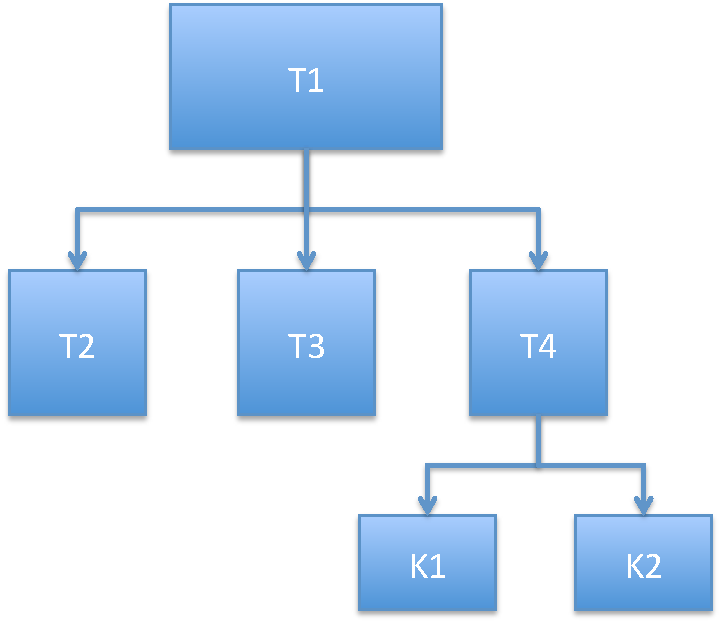
\includegraphics[scale=0.5]{figures/SimpleHierarchy.pdf}
\parbox{6in}{\caption{A simple processing network.\label{simple_hierarchy_fig}}}
\end{figure}

In more detail, the rules of this policy are:
\begin{enumerate}
\item no data is passed (taken) laterally,
\item passing data between levels of the hierarchy must be explicit,
\item that lower elements use data objects provided by the higher levels,
\item that higher elements do not access objects created by lower elements,
\item and that lower elements do not use data objects from siblings.
\end{enumerate}

Refering to the diagram in Fig.~\ref{simple_hierarchy_fig}, we could immediately infer the following constraints:
\begin{enumerate}
\item T3 can use read/write data provided by T1;
\item T3 cannot use any data created by T2, nor any data provided by T1 to T2, unless T1 happens to provide that data to T3 as well;
\item T1 could not use data created by T3;
\item K2 could use data provided by T4;
\item The only way that K2 could use data provided by T1 would be if T4 explicitly relayed it to K2.
\end{enumerate}



%  FleCSI Data Requirements: Field requirementes section.

\section{Field Requirements}\label{FieldRequirementsSec}

\subsection{Use Cases}

\begin{table}[hbt]
\begin{tabular}{c p{5 in}}
\toprule
Use Case & Description \\
\midrule
\useNumber & adds a field on request: adds metadata, associates metadata to field\\
\useNumber & allocates the FieldData corresponding to the field in the right memory\\
\useNumber & provides accessors to field data\\
\useNumber & deletes a field\\
\useNumber & deletes FeildData\\
\useNumber & retrieves a field\\
\useNumber & searches fields for matching metadata\\
\bottomrule
\end{tabular}
\centering
\parbox{5in}{\caption{Use cases for DataStore\label{data_store_field_use_case_table}}}
\stepcounter{useTable}
\end{table}


\begin{table}[hbt]
\begin{tabular}{c p{5 in}}
\toprule
Use Case & Description \\
\midrule
\useNumber & Is given read or write access to a field\\
\useNumber & updates a field\\
\useNumber & can declare or initialize a field\\
\useNumber & associates a field with an index set (dense or sparse) \\
\bottomrule
\end{tabular}
\centering
\parbox{5in}{\caption{Task/Driver use cases for Fields.\label{task_field_use_case_table}}}
\stepcounter{useTable}
\end{table}


\subsection{Field Requirements}

% \begin{table*}[!hbt]
% \begin{tabular}{c p{5 in}}
\begin{longtable}{c p{5 in}}
\caption[]{Requirements for Fields\label{data_field_req_table}}\\
\toprule
Requirement & Description \\
\midrule
\endfirsthead
\caption[]{(cont.) Requirements for Fields}\\
\toprule
Requirement & Description \\
\midrule
\endhead
\bottomrule[1.2pt]
\endfoot
\bottomrule[1.2pt]
\endlastfoot
% Association with metadata
& \emph{Metadata} \\
% name
\reqNumber & Associate a name with every Field.\\
& \emph{\tab[0.5cm]Discussion: Does the name need to be unique? Currently, the name is a unique identifier. It's not clear that that needs to be the case, though. For example, can there be a density field for all materials combined (hydro view), and a density field associated with chocolate, peanut butter, etc (chemistry view)? But if there are multiple fields with the same name, how does two packages refer to the same field? Namespacing?}\\
% namespace
\reqNumber & Associate a namespace with every Field.\\
& \Note{1}{The namespace can be defaulted.}\\
& \Note{2}{A name can occur zero or once in a namespace.}\\
% version
\reqNumber & Associate a version with each field.\\
& \Note{1}{This may be required for techniques like predictor-corrector methods.}\\
& \Note{2}{The version distinguishes between multiple instances of the same field name.}\\
& \Example{'pressure after time step 42' versus 'pressure after time step 43'.}\\
& \Discussion{Name, namespace, and version uniquely identify a field.} \\
% Id
\reqNumber & Associate a unique integer identifier with each field.\\
& \Example{We want to be able to talk about a data object independently of its name.}\\
& \Note{1}{an id would be more convenient than specifying name, namespace, and version.}\\
% builtin metadata
\reqNumber & Associate Fields with various builtin metadata aspects.\\
& \Note{1}{a field can be associated with 0 or more materials, 0 or more isotopes.} \\
% user-defined metadata
\reqNumber & Permit users to register metadata in the form of $<$Key,Value$>$ pairs.\\
& \Note{1}{Also permit users to search for and set user--define $<$Key,Value$>$ metadata.}\\
% Search, set
\reqNumber & Search for Fields matching a given metadata criterion.\\
\reqNumber & Set each metadata attribute for each Field.\\
\midrule

% Association of fields & topological elements
& \emph{Topological Elements} \\
\reqNumber & Associate Fields with homogeneous sets of elements of one mesh. \\
& \Note{1}{``homogeneous": only one type of element in the set.} \\
& \Note{2}{a field may be associated with any subset of the elements of a mesh, including all of the elements of that type on the mesh;} \\
& \Note{3}{a field need only be associated with the elements of one mesh.} \\
& \Note{4}{Arbitrary mesh entities, including cell centers, edges, faces, vertices, corners, wedges.}\\

% Association of fields and data
\midrule
& \emph{Data Elements} \\
\reqNumber & Associate fields with FieldData, i.e. the actual data.\\
& \Note{1}{There is a bijective relationship between Fields and FieldDatas.}\\
& \Note{2}{The type of FieldData is fairly arbitrary; it probably includes any type with a null constructor---any type that can be allocated via a new [] statement. Further specification is required.}\\
\reqNumber & Given a field descriptor, get read and write access to the FieldData.\\
& \Note{1}{Read access may be separated from write access.}\\
& \Note{2}{It would be nice to have a way of saying "done writing this field".}\\
\reqNumber & Associate each Field with an IndexSet.\\
& \Note{1}{Exactly one IndexSet per Field.}\\
% & \emph{}
% Initialization and persistence requirements



% Tracking

% \end{tabular}
\stepcounter{reqTable}
\end{longtable}
% \centering
%\parbox{5in}{\caption{Requirements for Fields}\label{data_field_req_table}}
% \end{table*}

Another key concept is the index set with which Field is associated.
The index set defines the subset of mesh entities to which the FieldData correspond.


% \clearpage
\subsection{FieldData}

FieldData are the actual variables associated with the mesh elements.
They represent physically or computationally interesting quantities.
The representation of these data is closely bound up with effecient iteration over them.
Requirements on these data need to be sensitive to the possibility of needing different views and different layouts of the data for different machines and different algorithms.

\begin{table}[hbt]
\begin{tabular}{c p{5 in}}
\toprule
Requirement & Description \\
\midrule
\reqNumber & This table should capture requirements for FieldData. \\
\bottomrule
\end{tabular}
\centering
\parbox{5in}{\caption{Requirements for accessing FieldData, getting to it, allocation it, initializing and persisting it.}\label{field_data_req_table}}
\stepcounter{reqTable}
\end{table}




%  FleCSI Data Requirements: particle requirementes section.

\section{Particle Requirements}\label{ParticleRequirementsSec}

Fields acquire strcuture naturally from the (sub)meshes with which they are associated.
Particles are not always so easily structured.
This requires care and maintenance in specifying requirements for particles.
We assume there will be some kind of organizing principle above the level of individual particles.
Thus we distinguish between:
\begin{enumerate}
\item ParticleSet, a descriptor of a set of particles,
\item ParticleData, space for recording the attributes of particles,
\item ParticleIndex, a ``virtual'' grouping of particles.
\end{enumerate}
\subsection{Use Cases}



\begin{table}[hbt]
\begin{tabular}{c p{5 in}}
\toprule
Use Case & Description \\
\midrule
\useNumber & adds a ParticleSet on request: adds metadata, associates metadata to particle\\
\useNumber & allocates the ParticleData corresponding to the particle in the right memory\\
\useNumber & provides accessors to particle data\\
\useNumber & deletes a particle set\\
\useNumber & deletes particle data\\
\useNumber & retrieves a ParticleSet\\
\useNumber & retrieves a ParticleData\\
\useNumber & searches ParticleSets for matching metadata\\
\bottomrule
\end{tabular}
\centering
\parbox{5in}{\caption{DataStore use cases for particles.\label{data_store_particle_use_case_table}}}
\stepcounter{useTable}
\end{table}


\begin{table}[hbt]
\begin{tabular}{c p{5 in}}
\toprule
Use Case & Description \\
\midrule
\useNumber & Is given read or write access to ParticleData\\
\useNumber & updates ParticleData\\
\useNumber & can declare or initialize a ParticleSet\\
\useNumber & can declare or initialize ParticleData\\
\useNumber & can declare or initialize ParticleIndex\\
\bottomrule
\end{tabular}
\centering
\parbox{5in}{\caption{Task/Driver use cases for particles.\label{task_particle_use_case_table}}}
\stepcounter{useTable}
\end{table}


\subsection{ParticleSet Requirements}

% % \begin{table*}[!hbt]
% % \begin{tabular}{c p{5 in}}
% \begin{longtable}{c p{5 in}}
% \caption[]{Requirements for Particles\label{data_particle_req_table}}\\
% \toprule
% Requirement & Description \\
% \midrule
% \endfirsthead
% \caption[]{(cont.) Requirements for Particles}\\
% \toprule
% Requirement & Description \\
% \midrule
% \endhead
% \bottomrule[1.2pt]
% \endfoot
% \bottomrule[1.2pt]
% \endlastfoot
% % Association with metadata
% & \emph{Metadata} \\
% % name
% \reqNumber & Associate a name with every Particle.\\
% & \emph{\tab[0.5cm]Discussion: Does the name need to be unique? Currently, the name is a unique identifier. It's not clear that that needs to be the case, though. For example, can there be a density particle for all materials combined (hydro view), and a density particle associated with chocolate, peanut butter, etc (chemistry view)? But if there are multiple particles with the same name, how does two packages refer to the same particle? Namespacing?}\\
% % namespace
% \reqNumber & Associate a namespace with every Particle.\\
% & \Note{1}{The namespace can be defaulted.}\\
% & \Note{2}{A name can occur zero or once in a namespace.}\\
% % version
% \reqNumber & Associate a version with each particle.\\
% & \Note{1}{This may be required for techniques like predictor-corrector methods.}\\
% & \Note{2}{The version distinguishes between multiple instances of the same particle name.}\\
% & \Example{'pressure after time step 42' versus 'pressure after time step 43'.}\\
% & \Discussion{Name, namespace, and version uniquely identify a particle.} \\
% % Id
% \reqNumber & Associate a unique integer identifier with each particle.\\
% & \Example{We want to be able to talk about a data object independently of its name.}\\
% & \Note{1}{an id would be more convenient than specifying name, namespace, and version.}\\
% % builtin metadata
% \reqNumber & Associate Particles with various builtin metadata aspects.\\
% & \Note{1}{a particle can be associated with 0 or more materials, 0 or more isotopes.} \\
% % user-defined metadata
% \reqNumber & Permit users to register metadata in the form of $<$Key,Value$>$ pairs.\\
% & \Note{1}{Also permit users to search for and set user--define $<$Key,Value$>$ metadata.}\\
% % Search, set
% \reqNumber & Search for Particles matching a given metadata criterion.\\
% \reqNumber & Set each metadata attribute for each Particle.\\
% \midrule

% % Association of particles & topological elements
% & \emph{Topological Elements} \\
% \reqNumber & Associate Particles with homogeneous sets of elements of one mesh. \\
% & \Note{1}{``homogeneous": only one type of element in the set.} \\
% & \Note{2}{a particle may be associated with any subset of the elements of a mesh, including all of the elements of that type on the mesh;} \\
% & \Note{3}{a particle need only be associated with the elements of one mesh.} \\
% & \Note{4}{Arbitrary mesh entities, including cell centers, edges, faces, vertices, corners, wedges.}\\

% % Association of particles and data
% \midrule
% & \emph{Data Elements} \\
% \reqNumber & Associate particles with ParticleData, i.e. the actual data.\\
% & \Note{1}{There is a bijective relationship between Particles and ParticleDatas.}\\
% & \Note{2}{The type of ParticleData is fairly arbitrary; it probably includes any type with a null constructor---any type that can be allocated via a new [] statement. Further specification is required.}\\
% \reqNumber & Given a particle descriptor, get read and write access to the ParticleData.\\
% & \Note{1}{Read access may be separated from write access.}\\
% & \Note{2}{It would be nice to have a way of saying "done writing this particle".}\\
% \reqNumber & Associate each Particle with an IndexSet.\\
% & \Note{1}{Exactly one IndexSet per Particle.}\\
% % & \emph{}
% % Initialization and persistence requirements



% % Tracking

% % \end{tabular}
% \stepcounter{reqTable}
% \end{longtable}
% % \centering
% %\parbox{5in}{\caption{Requirements for Particles}\label{data_particle_req_table}}
% % \end{table*}

% Another key concept is the index set with which Particle is associated.
% The index set defines the subset of mesh entities to which the ParticleData correspond.


% \clearpage
\subsection{ParticleData}

% ParticleData are the actual variables associated with the mesh elements.
% They represent physically or computationally interesting quantities.
% The representation of these data is closely bound up with effecient iteration % over them.
% Requirements on these data need to be sensitive to the possibility of needing % different views and different layouts of the data for different machines and % different algorithms.
%
% \begin{table}[hbt]
% \begin{tabular}{c p{5 in}}
% \toprule
% Requirement & Description \\
% \midrule
% \reqNumber & This table should capture requirements for ParticleData. \\
% \bottomrule
% \end{tabular}
% \centering
% \parbox{5in}{\caption{Requirements for accessing ParticleData, getting to it, % allocation it, initializing and persisting it.}\label{particle_data_req_table}}
% \stepcounter{reqTable}
% \end{table}




%  FleCSI Data Requirements: Physical Data requirementes section.

\section{Physical Model Data Requirements}\label{PhysicalModelRequirementsSec}

Physical models are used to represent physics that is too expensive to compute on--the--fly.
Instead, that data is typically stored in tabular form.
Many tables may be required in the course of a simulation.
This section captures the requirements for such data.

\begin{table}[hbt]
\begin{tabular}{c p{5 in}}
\toprule
Requirement & Description \\
\midrule
\reqNumber & This needs more specification \\

\bottomrule
\end{tabular}
\parbox{5in}{\caption{Requirements for Physical Model Data}\label{phys_data_req_table}}
\stepcounter{reqTable}
\end{table}



%  FleCSI Data Requirements: Simulation Launch configuration data requirementes section.

\section{Static Simulation Configuration Data Requirements}\label{SimConstRequirementsSec}

Certain data is specified at simulation launch time; it remains static throughout the run.
This data may be required throughout the simulation.
It may include physical data, such as the domain extents, or
computational data, such as the starting time step, or the (static)
configuration of the run.
This data excludes things that change over the course of the simulation,
 such as current simulation time, or current mesh partition.

\begin{table}[hbt]
\begin{tabular}{c p{5 in}}
\toprule
Requirement & Description \\
\midrule
\reqNumber & This needs more specification \\

\bottomrule
\end{tabular}
\parbox{5in}{\caption{Requirements for Simulation Launch Data}\label{sim_launch_data_req_table}}
\stepcounter{reqTable}
\end{table}



%  FleCSI Data Requirements: Simulation State Data requirementes section.

\section{Mutable Simulation Configuration Data Requirements}\label{SimMutableRequirementsSec}



\begin{table}[hbt]
\begin{tabular}{c p{5 in}}
\toprule
Requirement & Description \\
\midrule
\reqNumber & Partition Data \\
\reqNumber & Cycle Information \\
& \Note{1}{to include: cycle number, cycle start time, delta-t, ... more spec needed}\\
& \Note{2}{should include data that can be registered and set by the user/package.}\\
& \Note{2a}{is granularity finer than cycle/time-step required?}\\
\bottomrule
\end{tabular}
\parbox{5in}{\caption{Requirements for Mutable Simulation State Data}\label{mutable_sim_state_data_req_table}}
\stepcounter{reqTable}
\end{table}

\begin{table}[hbt]
\begin{tabular}{c p{5 in}}
\toprule
Requirement & Description \\
\midrule
\reqNumber & Communications topology \\
& \Note{1}{There may be multiple partitions of a single mesh.}\\
& \Note{2}{There may be multiple meshes, each partitioned differently.}\\
\bottomrule
\end{tabular}
\parbox{5in}{\caption{Requirements for Partitioning Data}\label{partition_data_req_table}}
\stepcounter{reqTable}
\end{table}



% \begin{thebibliography}{10}
% \end{thebibliography}

~\verb+__________________+

\closing

\end{document}

%%---------------------------------------------------------------------------%%
%% end of <papername>.tex
%%---------------------------------------------------------------------------%%
